% !TeX spellcheck = cs_CZ
\chapter{Testování}
\label{chap:testovani}
V průběhu vývoje a testování jsem využíval nástroje Wireshark pro sledování síťového provozu mezi útočníkem a obětí. Všechny útoky byly testovány na běžné uživatelské stanici s operačním systémem Linux, konkrétně Fedora 27. Tato stanice sloužila pouze jako generátor útoků. Stanice vystupující při útoku jako \uv{reflektor} nebo \uv{amplifikátor} a \uv{oběť} jsou plně virtualizované operační systémy skrze hypervizor kernelu (KVM) přistupující ke stejnému síťovému rozhraní \texttt{vnet0}, na něž je připojena i hostitelská stanice. Toto rozhraní je od internetu odděleno prostřednictvím NAT. Pro snazší správu virtualizovaných stanic bylo použito aplikace Virtual Machine Manager ve verzi 1.4.3.

\section{Testování útoku NTP Flood}
Operační systém na kterém je spuštěn NTP sever jsem musel zvolit Fedora 14 jejíž datum vydání bylo 2.\ 11.\ 2010. Bylo nutno zvolit takto starou verzi z důvodu opravy chyby v balíčku \texttt{ntp} v pozdějších vydáních. Nainstalován byl tedy balí \texttt{ntp-4.2.6p3}. Na tomto stroji musel být správně nakonfigurován firewall tak, abych byl schopen službu NTP kontaktovat z jiné stanice. Následně byl změněn konfigurační soubor pro NTP server způsobem popsaným v kapitole \ref{subsec:ntp_flood}.

Na serveru, který slouží jako oběť tohoto útoku je spuštěn operační systém Fedora 26 Server a nainstalován Apache server ve verzi \texttt{httpd-2.4.29}. Firewall je také patřičně nakonfigurován.

Dalším krokem je vygenerování falešných uživatelů dotazujících se na NTP server. To provedeme spuštěním skriptu a následně si můžeme ověřit pomocí příkazu \texttt{ntpdc}, že záznamů je požadované množství.
%TODO:dependence skriptu, popsat instalaci
\begin{lstlisting}
python3 fake_ntp_hosts.py
ntpdc -n -c monlist 192.168.124.14 | wc -l
\end{lstlisting}

\noindent V tomto okamžiku nic nebrání spuštění útoku a to následovně:
\begin{lstlisting}
./dosgen -i virbr0 -P 4 --ntp -s 192.168.124.129 \
	-d 192.168.124.14
\end{lstlisting}

Nyní je NTP server zahlcován dotazy. Odpověďi na ně zasílá na IP adresu oběti. Výstup aplikace DoSgen lze vidět na obrázku \ref{fig:dosgen_run_ntp-img}

\begin{figure} [ht]
	\centering
	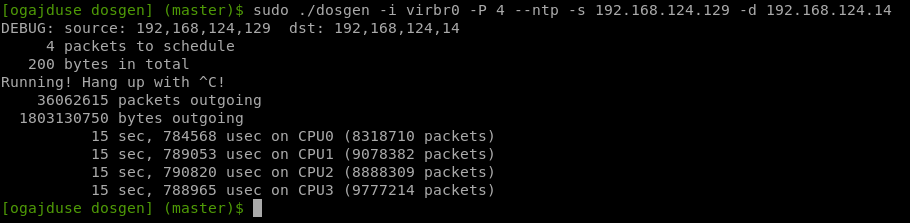
\includegraphics[width=0.9\textwidth]{obrazky/dosgen_terminal_run_ntp.png} %.pdf
	\caption{Spuštění aplikace DoSgen se zvoleným NTP útokem}
	\label{fig:dosgen_run_ntp-img}
\end{figure}

Při sledování provozu v programu Wireshark můžeme vidět, že na NTP server je vyslán požadavek \uv{monlist} a NTP server na něj odpovídá, přičemž zamění zdrojovou adresu zamění za cílovou a naopak a paket je tak vyslán na server oběti, která o něj nejeví zájem, tudíž na každý z nich odpovídá ICMP zprávou typu 3 s kódem 9 (Host administratively prohibited). Server je tak zaměstnán odesíláním těchto zpráv a je tedy vyčerpána šířka pásma, dochází k DoS útoku.

\begin{figure} [h]
	\centering
	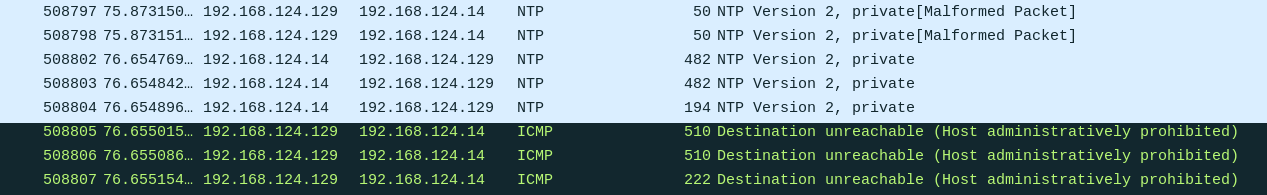
\includegraphics[width=0.9\textwidth]
	{obrazky/mon_getlist_1_wireshark_with_icmp_and_reply.png}
	\caption{Spuštění aplikace DoSgen se zvoleným NTP útokem}
	\label{fig:mon_getlist_1_wireshark_with_icmp_and_reply-img}
\end{figure}

Celá tato komunikace je zachycena na obr. \ref{fig:mon_getlist_1_wireshark_with_icmp_and_reply-img}. Pakety s číslem 508797 a 508798 jsou vygenerované nástrojem DoSgen. Následující tři pakety, tedy pakety s číslem 508802-508804 jsou odpovědí NTP serveru. Tato odpověď obsahuje pouze 13 hostů, v případě, že nám server vrátí 600 hostů, odpověď od serveru bude mnohonásobně větší.

Nutno poznamenat, že na serveru oběti musela být uměle modifikována šířka pásma a to na 100 Mbit/s v obou směrech.






%ntpdc -n -c monlist 3.cz.pool.ntp.org